
% This is LLNCS.DEM the demonstration file of
% the LaTeX macro package from Springer-Verlag
% for Lecture Notes in Computer Science,
% version 2.4 for LaTeX2e as of 16. April 2010
%
\documentclass{llncs}
%
\usepackage{makeidx}  % allows for indexgeneration
\usepackage{graphicx} % so we can include images
\usepackage{inputenc} % display all characters properly
\usepackage[english,american]{babel}

\usepackage{url}
\usepackage{listings} % for listing code
\usepackage{color} % colors are nice

\definecolor{black}{rgb}{0,0,0}
\definecolor{gray}{rgb}{0.6,0.6,0.6}
\definecolor{white}{rgb}{1,1,1}

\definecolor{keywords}{rgb}{0.5,0,0.6}
\definecolor{strings}{rgb}{0,0.4,0}
\definecolor{comments}{rgb}{0.5,0.5,0.5}

\newcommand{\comment}[1]{}
\definecolor{Orange}{rgb}{1,0.5,0}
\newcommand{\todo}[1]{\textsf{\textbf{\textcolor{Orange}{[#1]}}}}

\lstset{
  language=Java,
  basicstyle=\ttfamily\footnotesize,
  numbers=left,
  numberstyle=\tiny\color{gray},
  stepnumber=1,
  numbersep=5pt,
  frame=single,
  tabsize=2,
  captionpos=b,
  breaklines=true,
  breakatwhitespace=true,
  keywordstyle=\color{keywords},
  commentstyle=\color{comments},
  stringstyle=\color{strings},
}

%
\begin{document}
%
\frontmatter          % for the preliminaries
%o
\pagestyle{headings}  % switches on printing of running heads
\addtocmark{Code Generation From ECDAR} % additional mark in the TOC
%
\mainmatter              % start of the contributions
%
\title{Code Generation From ECDAR}
%
\titlerunning{Code Generation From ECDAR}  % abbreviated title (for running head)
%                                     also used for the TOC unless
%                                     \toctitle is used
%
\author{Rasmus Berntsen \and Florian Biermann \and Lauge Groes \and Nicolas Wainach Lundqvist Jensen \and Thomas Kokholm \and Piort Stawiski \and Wiktor Michal Zdziechowski}

\authorrunning{Rasmus Berntsen et al.} % abbreviated author list (for running head)

%%%% list of authors for the TOC (use if author list has to be modified)
\tocauthor{Rasmus Berntsen, Florian Biermann, Lauge Groes, Nicolas Wainach Lundqvist Jensen, Thomas Kokholm, Piort Stawiski, Wiktor Michal Zdziechowski}

\institute{IT University of Copenhagen, Denmark\\
\email{\{raber, fbier, lgro, nicl, tkok, psta, wmic\}@itu.dk}
}
\maketitle % typeset the title of the contribution

\begin{abstract}
This paper present a framework for code generation, based on timed automatas modelled in ECDAR (Environment for Compositional Design and Analysis of Real Time Systems). A graphical tool based on UPPAAL that allows to visually create models of real-time systems.

A key feature missing in ECDAR is the possibility to utilize models for code generation, as way to develop software solutions based on visually represented models.

This project introduces how java code is generated from an ECDAR model. It also introduce the notation of tasks as an extension to the ECDAR model within the framework.

The functionality of the framework is evaluated through a series of test. All of which is based on beverage-serving machine model (See figure \ref{bev-machine} on page \pageref{bev-machine}).


\todo{Introduce tasks:
At man kan placere en opgave på forskellige lokationer.
}
\todo{Define problemstatement:
A kunne udnytte modeller til at genere code til en 
}
\todo{Tell about our solution:
Vores framework der generere java code ud fra automatas i ecdar filen
}

\end{abstract}


\section{Introduction}
\label{introduction}
In the preceeding years a new level of abstraction in development have been evolving. Utilizing a higher level of abstraction, than high-level programming languages, we have Model Driven Development. This new paradigm is combining a focus on automatisation and code generation, to enable a new way of black boxing solutions within a multitude of specialists outside traditional programming while securing platform independency.  

\subsection {Real Time Computing \label{introduction-rts}}
%
Real-time computing is the study of hardware and software systems that must satisfy explicit 
response-time constraints or risk severe consequences, including failure. Timed systems are 
used in a wide range of domains including communications, embedded systems, real-time and automated control. 
They can be easily found in our environment; one of simple examples is the airbag system in a car. 
The real-time constraint in this system is the reaction time between crash sensors receiving input and 
the deployment of airbags. Among some of the important characteristics of real-time systems we can distinguish 
extreme reliability and safety as they are very often safety-critical.    

\subsection{ECDAR \label{introduction-ecdar}}
%
The “Environment for Compositional Design and Analysis of Real Time Systems” (ECDAR) - is a graphical tool based on UPPAAL TIGA \cite{behrmann_uppaal-tiga:_2006} that 
allows to visually create models of real-time systems. Unlike UPPAAL \cite{larsen_uppaal_1997}, it is implementing a complete specification theory for 
real time systems \cite{David:2010:TIA:1755952.1755967,conf/atva/DavidLLNW10}. In ECDAR, components of the system are described as automatons extended with clocks (timed automata), 
that can be combined to form larger comprehensive system descriptions. Correct specification of composition is supported by 
well defined compositional reasoning theory, consisting of operators like: parallel composition, conjunction, satisfaction 
checking and refinement. On the top of that, the tool allows for scalable verification of models by querying the 
implementation with verification questions \cite{conf/atva/DavidLLNW10}.
%

\subsection{Project \label{introduction-problemfield}}
This paper will follow an implementation of code generation from ECDAR to Java. The proposed implementation of the ECDAR code generator is split up in two parts. The first part is a framework of abstract classes, implementing in as much detail as possible the single parts of ECDAR specifcations (i.e. edges, locations, TIOA). The second is the actual code generation. Our code generator generates sources which inherit from the abstract framework to minimize the amount of code that needs actually to be generated.
The paper will also detail the different testing issues and benefits of implementing code generation for TIOA, and reflect upon how this could be implemented concretely for Real Time Systems. 

\begin{itemize}
\item Simple extension of ECDAR
\item Design of the code generated software
\item Including a runtime framework and model framework completion
\item Some test plan
\item Analysis and criteria of Java RT
\end{itemize}



\section{Background}
\label{background}
%% BACKGROUND (Wiktor) %%% 

% LAST UPDATE: applying changes from Andrzej's comments (27.11.2012) % 


\subsection{Timed Input/Output Automata \label{background-tioa}}
%
The "Timed Input/Output Automata" is a basic, mathematical specification framework for description and analysis of real time systems. 
In this framework, system is represented by nondeterministic, possibly infinite-state, state machine referred 
as “timed I/O automaton” (TIOA) \cite{Kaynar:2006:TTI:1203437}. TIOA has been implemented as the modeling language in ECDAR \cite{conf/atva/DavidLLNW10}.

\begin{figure}[t]
\label{simple-model}
\begin{centering}
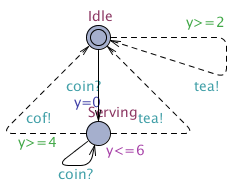
\includegraphics[scale=0.7]{images/bev_machine_model}
\par\end{centering}
\caption{Model of beverage-serving machine.}
\label{bev-machine}
\end{figure}

The preceding figure (see fig. \ref{bev-machine}) illustrates the model of beverage-serving machine. Given a coin (\emph{coin}), it serves either coffee (\emph{cof}) 
or tea (\emph{tea}) within a given time interval. Moreover, free tea is served once in awhile. In the example, the TIOA consists of and two locations represented by 
circles: \emph{Idle} and \emph{Serving}. \emph{Idle} represents the starting location, and the state of machine waiting for coin input (\emph{coin?}).  
 The flow of TIOA is controlled by three types of labels: \emph{invariants}, \emph{guards} and \emph{clock-reset operations}. 
Invariants are defined on locations ($y\leq 6$) and represent constraints for the clocks in order for the control to remain in particular location until time requirement is fulfilled.  
Guards are located on the edges ($y\geq 2$ and $y\geq 4$) and express conditions on the values of clock that must be satisfied in order for 
the edge to be taken. When the condition is satisfied, the transition occurs and action (\emph{cof!} or \emph{tea!}) is triggered. Clock-reset operations ($y=0$) are simple
clock value manipulations in form of assignment that enforce progress in the system.

In ECDAR, the specification interface is leveraging the UPPAAL TIGA language \cite{behrmann_uppaal-tiga:_2006} to describe TIOA. However, the following constraints are retained\footnote{See \href{http://people.cs.aau.dk/adavid/ecdar/examples.html\#lang}}:   
%
\begin{itemize}
\item Invariants may not be strict.
\item Inputs must use controllable edges.
\item Outputs must use uncontrollable edges.
\item All channels must be declared broadcast.
\item The system is implicitly input enabled due to broadcast communication but for refinement checking purposes the relevant inputs must be explicit in the model.
\item In the case of parallel composition of several components, a given output must be exclusive to one component.
\item For implementations, outputs must be urgent.
\item For implementations, every state must have independent time progress, i.e., progress must be ensured by either an output or infinite delay.
\item $\tau$-transitions (no output or input) are forbidden. %There was a comment about this item%
\item Global variables are forbidden.
\end{itemize}

\subsection{Code Generation \label{background-codegeneration}}
In order to clarify what code generation is one need to understand what a model transformation is, as this is a fundamental part of code generation. In short one could say that the model transformation is a way to ensure that the final code is consistent and with a reduced number of errors. The generation is an automated way to produce code from models. The actual generation is defined by the software developer, thus it is defined what the output should be, but the input and the data is not.

There is generally two ways to do model transformations, that is model to model and model to text, the former known as M2M and the latter M2T. There are also a lot of other tools and techniques for transformation, which should not be confused with model transformations. One could mention an XSLT-transformation as an example, where the base input is an XML-document and the final output is another XML-document, often XHTML, with a predefined XML-Schema.

Model to model is a transformation of a number of models to a given number of new models - from X number of models to Z number of new models. Model to text is the transformation of a number of models to text, the text could for instance be code - which is why the process sometimes is known as model to code.





\section{Implementation}
\label{implementation}
The proposed implementation of the ECDAR code generator is split up
in two parts. The first part is a framework of abstract classes, implementing
in as much detail as possible the single parts of ECDAR specifications
(i.e. edges, locations, TIOA). The second is the actual code generation.
Our code generator generates sources which inherit from the abstract
framework to minimize the amount of code that needs actually to be
generated. This means that nearly all design decisions have been made
prior to generating code, reducing space for possible errors. This
section describes our implemented subset of ECDAR and the code generator
in detail.

\subsection{Tasks}

ECDAR defines the behavior of a system as a state machine. This behavior
is, however, still too abstract to justify code generation. We can
generate code which implements the behavior of state machines, but
in essence, the system would then only produce messages.

To make this tool more useful, we introduce the notion of tasks as
an extension to the language. Let $T_{S}$ be a set of tasks and $L_{S}$
a set of locations on a system $S$. Then $\forall l\in L_{s}\exists t\in T_{s}$,
i.e. each location is assigned exactly one task. A task is a procedure
which will be executed as soon as an automaton traverses over an edge,
arriving at a new location.

Tasks can either be preemptive or non-preemptive. This property becomes
important for defining behavior of automata when they are notified
about input by the controller.

ECDAR is input-enabled (see Sect. \ref{background-ecdar}) and therefore,
the system is required to react to input immediately. As a consequence,
there must also be a well defined reaction to input during the execution
of a task.

When an automaton is executing a task and it receives an input message
which it accepts, it may stop the currently executed task and proceed
as originally defined in ECDAR (i.e. traverse the corresponding edge),
if and only if the task is preemptive. Otherwise, the given input
will be ignored and the execution of the task continues.

To determine if a task is preemptive is up to the designer of the
system to decide. By default are all tasks non-preemptive.

\subsection{The ECDAR Framework \label{implementation-framework}}

\begin{figure}[t]
\begin{centering}
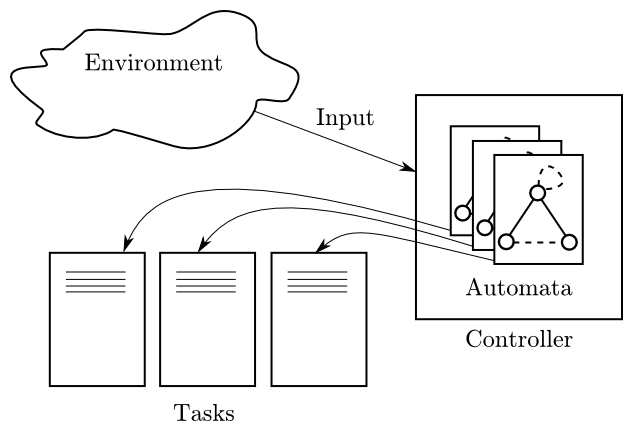
\includegraphics[scale=0.5]{images/ecdar_architecture} 
\par\end{centering}

\caption{Schematic of the architecture of our ECDAR implementation.}
\end{figure}

The architecture we chose is based upon the work of Amnell et al.\cite{amnell_code_2002}
with some modifications. Communication between automata is implemented
as message passing between environment and automata, where automata
send messages to the environment by traversing over output edges --
there are no shared variables (see Sect. \ref{background-tioa}). Messages
are processed by a controller object, which initializes automata and
also notifies automata about received messages.

We require multiple automata to execute in quasi-parallel. Therefore,
we do not queue tasks. Since the automata are moved to classical threading
architecture, we do not require multiple processor units. Instead,
the controller and each automaton run in separate threads. Since there
is no communication between automata directly, we can minimize synchronizing
so that nearly no waiting is required.

The following overview will give further implementation details on
each component of ECDAR as we implemented it. Each component is illustrated 
with a short code example, implementing ECDAR's "University" example%
\footnote{\href{http://people.cs.aau.dk/adavid/ecdar/examples.html\#university}}%
. For clarity, we omit the framework implementation and focus on the generated
code.

\subsubsection{Locations.}

Each location is a associated with a task. Task execution is implemented
in a separate thread, not blocking the execution of the automaton.
Locations are implemented as objects holding an array of edges that
point away from it. (See Fig. \ref{location-example})

\begin{figure}[t]
\lstinputlisting[linerange={101-132}]{code/Machine.java}
\caption{Example of location code. \label{location-example}}
\end{figure}


\subsubsection{Edges.}

An edge holds a reference to the location which the parent automaton
will be at after traversing this very edge. Edges can be asked if
they will be available at a given time. This is implemented to enable
lazy waiting in the automaton's traversal checker. Each edge is associated
with some input. If an edge is controllable, it will be triggered
if the automaton is notified at this input. If it is uncontrollable,
it will send its input to the controller. Furthermore, edges have
access to the clock of the parent automaton to reset it appropriately.

The implementation makes a class-wise distinction between controllable
and uncontrollable edges and hard-codes the behavior for given input.
Such hard-coded features are e.g. notifying the controller on traversing
an uncontrollable edge. (See Fig. \ref{edge-example})


\subsection{TIOA.}

The implementation of timed I/O automata holds a set of locations
and a reference to the location it is currently at. The TIOA is executed
by a thread that keeps checking for available edges and traverses
along these, as soon as they become enabled. To check if an edge is
available, let $E_{s\rightarrow t}$ be an edge where $s,\, t$ are
start and target locations respectively. Furthermore, let $g(E)$
be a function evaluating the guard of an edge $E$ and $I(l)$ a function
evaluating the invariant of a location $l$. Our implementation uses
$g'(E_{s\rightarrow t})=g(E_{s\rightarrow t})\wedge I(t)$ to check
if $E_{s\rightarrow t}$ is available.

Additionally, the automaton has the ability to return the current
local clock state (see \ref{implementation-presumptions}) and to
reset the clock. We use the same notion of clocks as \cite{amnell_code_2002},
where time on the local clock is the difference between the current
time on the system clock and the time the local clock was started.
Resetting the local clock means to use the current system clock time
as the new start time. (See Fig. \ref{tioa-example})

\begin{figure}[t]
\lstinputlisting[linerange={8-8,169-184}]{code/Machine.java}
\caption{Example of TIOA code. \label{tioa-example}}
\end{figure}


\subsubsection{Controller.}

The controller holds all automata given in the specification, executes
them initially in quasi-parallel and notifies automata about input
from the environment. It is a singleton, accessible in a static fashion.
This property is useful for uncontrollable edges that need to notify
the controller about input. (See Fig. \ref{controller-example})

\begin{figure}[t]
\lstinputlisting[linerange={6-11,63-64}]{code/UniversityController.java}
\caption{Example of controller code. \label{controller-example}}
\end{figure}


\subsection{Synchronization}

In the framework implementation, the Java keyword \textit{synchronized} is 
used for making certain operations quasi-atomic. That means, that a set of
instructions may not be interrupted by the execution of another thread -- 
i.e. traversals over edges.

This is mainly used for the logging of signals, so that logging time
is preserved and the output appears in the right order. \textit{Synchronized}
is also used, to set some internal states on TIOA, where the internal state
consists of multiple values that need to be set at the same time.

\textit{Synchronized} is furthermore used to prioritize handling of input.
The method on the controller object, that is handling the signal, as well as
those on the TIOA that react to a signal if it is accepted, are modified with
\textit{synchronized}. This ensures that, before everything else, the input
is processed.


\subsection{Code Generation \label{implementation-code-generation}}
In our implementation the actual generation of our source code is done through a model to text Transformation. Our base model is the input from the ECDAR file and the final generation is resulting in compilable JAVA-files based on this input. The method of transformation is known as "Model To Text", as in our example we transform a model, ECDAR, into text, JAVA. So what we are actually doing is generating code from an abstract model from ECDAR and turn it into a lower level of abstraction, in this case JAVA. We will from here solely focus on model to text, as this is the transformation we chose.
\newline

We use the Eclipse Modeling Framework (EMF) which is a modeling framework and code generation facility for building applications based on a structured data model. From a model specification described in XMI, EMF provides tools and runtime support to produce a set of Java classes for the model, along with a set of adapter classes that enable viewing and command-based editing of the model, and it provides a basic editor.
The core EMF framework includes a meta model (Ecore) for describing models and runtime support for the models including: change notification, persistence support with default XMI serialization, and a very efficient reflective API for manipulating EMF objects generically. From the ECDAR Ecore model we generate an Xtext environment. Xtext is a framework for development of programming languages and domain specific languages. 
\newline
In order to generate code from our model we need to go through a process of multiple steps: We need to get our input from ECDAR, translate this to Xtext ECDAR DSL, we need a workflow that manages the process and finally need a XPAND-template that defines how the transformation should look. Each step is described in the following sections.

The generated output from the ECDAR enviroment is XML-files, which contains a complete definition of the model, with locations, edges, variables, transformations etc. In order to work with these files and do the actual code generation, we need to convert them to the Xtext ECDAR DSL. For this conversion we have a converter that simply takes the ECDAR XML-file and converts it to ECDAR DSL. The ECDAR DSL syntax is defined in EcdarText.xtext. With the combination of our Ecore meta model and our Xtext syntax we can define a workflow describing how to handle the generation process. We do this with the help of the Modeling Workflow Engine 2 (MWE2). Also defined in the workflow is the template that describes how the actual output is going to look like. The templates are written using Xpand. Xpand is a statically typed template language. Conveniently Xpand supports code-completion directly connected to the Ecore model defined in the MWE2 workflow, not to talk about syntax coloring, refactoring and error highlighting. For our implementation we have ended up with having serveral workflows and templates to do the rather complex transformations: One set of workflows and templates for respectively the Specification, Controller and Environment.

In the workflow-file one defines what model to use, a slot-name to refer to later and an entry point. The entry point defines which class element is the top, or root, element. Our entry-element is "ETSpecificationDefinition". Also defined in the workflow is how we are going to use the entry-element. For instance in our specification workflow we have defined that for each "ETSpecificationDefinition" we do a transformation using the Xpand template for this particular task. We then end up with having generated ouput for each specification that was initialy described and modeled from within the ECDAR XML-file.

With the workflow fully configured, the next step is to write the transformation. This is done in a Xpand template. The snippets in figure \ref{xpand-example} shows some important steps.

\begin{figure}[t]
\lstinputlisting[linerange={1-2}]{code/TemplateSpecifications.xpt}
\lstinputlisting[linerange={6-6}]{code/TemplateSpecifications.xpt}
\lstinputlisting[linerange={34-41}]{code/TemplateSpecifications.xpt}
\caption{Snippets from Xpand-template \label{xpand-example}}
\end{figure}

The arrows, known as guillemets ("«" & "»"), shows where in figure \ref{xpand-example} we use the XPAND language. First of all we import our model in the first line, referenced as ecdarText. We then proceed to one of the central concepts of Xpand by using the define-block; This is where we define our template. We only use one template is this specific file, but it could have contained multiple, which would have resulted in multiple define-blocks. In the next and last snippet we jump to a part where we are iterating through each edge and create a constructor for the current class. In the first line we create the constructor by inserting the text "Edge" and add the number the iterator has reached. We then iterate through a list of the current Edges variables, which should be one signal, and returns the results as a list. We furthermore use a new iterator to keep track of this itereation. We afterwards check if it's the first iteration, and if it is, we print out the edges target name and the variable signal, such as "super(C, "signal");".

The notion of tasks as previous described in section 3.2. is accounted for in our generated output. In the controller we generate functions that will be invoked at each location. A task is a procedure which will be executed as soon as an automaton traverses over an edge, arriving at a new location. There can only be one task pr. location. The thought behind having all methods in the controller is for a better overview and a centralized customizeable file.



\section{Evaluation and Discussion}
\label{evaluation}
\subsection{Testing}
\label{Testing}
In order to test our software solution three different testing methods have been arranged.

\subsubsection{Compiling properly}
Making sure every output compiles properly.

\subsubsection{Logfile testing}
For the project an logfile analysis program have been incorporated. A small program verifying that the signals in the generator code are fired in the right order according to the input model. 
The analysis program is hardcoded to match our testing model (see figure~\ref{simple-model} on page~\pageref{simple-model}). Thus it is checking for signals like: GRANT, COIN and TEA, in the specifyied order. If a signal is called within the generator before it is supposed too (e.g TEA before COIN) the analysis program will call for an ERROR. 

The logfile contain timestamps of global time from each atomaton in a model. The global time can then be verified by comparison with time assigned within the ECDAR modelling tool.

\subsubsection{Manual Comparison}
Final testing procedure is a manual step-by-step comparison of a simple graphical atomaton model and the corisponding code generated. Cycling through the times, comparing each step with the output.
%(verified by Andrzej Wasowski).

\subsection{Presumptions and Resulting Motivations\label{implementation-presumptions}}

Our implementation represents only a subset of actual ECDAR. Currently,
the implementation assumes only one clock per automaton. Also, we
assume the specification to be valid, since there are other tools
that verify correctness%
\footnote{\href{http://people.cs.aau.dk/adavid/ecdar/}%
}.

The only operator we implement for code generation is the parallel
composition operator. Let $M$ be the type ECDAR specification. Then
all operators in ECDAR are of type $M_{i}\otimes M_{j}\rightarrow M_{ij}$.
Other than for the majority of operators, which refine the specification,
it is impractical to implement parallel composition as a model-to-model
transformation, since it produces the cross-product of two models
\cite{david_compositional_2012}. These models are size $|M_{i}|\cdot|M_{j}|$
and generating code for them would consume a large amount of memory
and raise complexity. This would be inappropriate for an embedded
system. We elaborate on this further in Sect. \ref{implementation-framework}.

ECDAR specifications are written on the assumption of the synchrony
hypothesis (see Sect. \ref{background-ecdar}) \cite{david_compositional_2012}.
This is an important property for code generation, as reasoning about
time differences in execution becomes unnecessary for the developer.
However, we still kept overhead low to achieve reasonable fast performance.

%To produce feasible code that would be able to run on embedded systems,
%we targeted Real-Time Java (Java RTS)%
%\footnote{\href{}{http://www.oracle.com/technetwork/java/javase/tech/index-jsp-139921.html}%
%}. Java RTS was designed to improve upon standard Java in terms of
%timing accuracy an real-time embedded systems.





\section{Related Work}
\label{related}
ECDAR is a TIOA modeler based on UPPAAL. A similar tool based on UPPAAL already exists. 

\paragraph{Times}
Times\footnote{\href{http://www.timestool.com}} is a tool for modeling and implementation of embedded systems. Times is a graphical simulator, in which a user can validate dynamic behavior of a system and see how tasks execute - much like Ecdar, but it can also do code-generation. However there is a difference between Ecdar and Times.

Looking at what are taking as input by the controller - Times simple takes a model and generates code. ECDAR: Synthesize models for you so to avoid “that” stage. In ECDAR you have the possibility to you use composition.

\paragraph{Composable Code Generation for Model-Based Development}
by Kirk Schloegel et al. present a framework for generating code\cite{composable-code-generation}. They emphasize how utilizing their framework, code generators aren't programs seperated from a correspnding graphical model as it often have been in the past. Our code generator isn't based on this framework, however their approch on developing code generators with focus on graphical models is related to our apporch with ECDAR. 

\paragraph{Code Synthesis for Timed Automata}
by Tobias Amnell et al. present a framework for the development of real-time embedded
systems\cite{Amnell:2002:CST:779110.779112}. Their work is sumulor to our project. In the article the illustrate how their framework is based on timed automatas and real-time tasks - relative to our concept with ECDAR.



\section{Conclusion}
In this project we have developed a code generator for a TIOA modeller: ECDAR. We have succesfully generated code from simplified model into Java. See section~\ref{Testing} on page~\pageref{Testing}.






\bibliographystyle{plain}
\nocite{*}
\bibliography{MDD.bib}

\appendix
\section{First Appendix}

\end{document}
